%$$$$$$$$$$$$$$$$$$$$$$$$$$$$$$$$$$$$$$$$$$$$$$$$$$$$$$$$$$$$$$$$$$$$$$$$$$$$$$$$
%Paragraph 2:Concurrent updates에 대한 연구
%$$$$$$$$$$$$$$$$$$$$$$$$$$$$$$$$$$$$$$$$$$$$$$$$$$$$$$$$$$$$$$$$$$$$$$$$$$$$$$$$
\newpage
\section{확장성 있는 자료구조 연구}
\label{sec:datarelated}
많은 확장성 있는 방법과 이를 이용하는 자료구조들은 업데이트 비율에 따라 서로 다른 성능을 가진다.
기존 연구들은 낮거나 중간 정도의 업데이트 비율에서는 새로운 확장성있는
기법~\cite{McKenney98}~\cite{Matveev2015RLU}~\cite{Harris2001Lockfree} ~\cite{Fomitchev2004Lockfree}
~\cite{Timnat2012}을 연구하거나 그 기법을 새로운 자료구조에 
적용~\cite{Arbel2014ConcurrentRCU}~\cite{Dodds2015SCT}~\cite{AustinTClements2012RCUBalancedTrees}을
하도록 시도하고 있다.

\subsection{확장성 있는 자료구조를 위한 동기화 기법}

\subsubsection{RCU}
확장성을 위한 대표적 동기화 기법인 RCU는 \textit{McKenney}와 \textit{Slingwine}에 의해 개발되었고, 
이 방법은 동기화 기법 때문에 발생하는 오버헤드를 최소화 시킬 수 있다. 
특히 RCU는 리더들을 보호하기 위해 사용하는 동기화 기법에 대한 오버헤드를 최소화 시킬 수 있다. 
오버헤드가 최소화 되는 이유는 동기화 기법이 캐시 일관성 트래픽 문제를 발생 시키는 전역 변수를 수정하지 않고, 
파티션된 퍼코어 메모리에 상태를 저장하는 방법을 사용하기 때문이다.
따라서 RCU는 리더들이 수행하는 락의 오버헤드가 적고, 여러 리더 스레드와
하나의 라이터 스레드가 병렬로 수행이 가능하므로 굉장히 높은 확장성을 가질 수 있다.
이러한 장점 때문에 RCU는 현재 리눅스 커널에서 가장 많이 사용되고 있는 동기화 기법 중 하나이다. 
RCU의 단점으로는 RCU의 리더에 비해 라이터가 수행하는 방법은 복잡하므로 라이터가 많아 질 경우 
성능이 저하되는 문제가 있다. 

\begin{figure}[h]
    \centering
    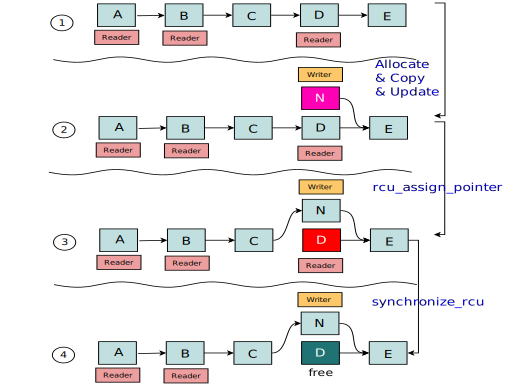
\includegraphics[width=1\textwidth]{fig/rcu/rcu_principle}
    \caption{RCU 예제}
  \label{fig:rcuprinciple}
\end{figure}

%$$$$$$$$$$$$$$$$$$$$$$$$$$$$$$$$$$$$$$$$$$$$$$$$$$$$$$$$$$$$$$$$$$$$$$$$$$$$$$$$
%Paragraph : RCU의 기본 철학
%$$$$$$$$$$$$$$$$$$$$$$$$$$$$$$$$$$$$$$$$$$$$$$$$$$$$$$$$$$$$$$$$$$$$$$$$$$$$$$$$
RCU의 기본 철학은 특정 시점에서 오브젝트를 복제해서 처리하는 것이다. 
그림~\ref{fig:rcuprinciple}은 이러한 RCU의 예를 보여준다.
먼저 그림에서 1단계에는 \code{A, B, C, D, E} 오브젝트 중 \code{A, B, D} 오브젝트를 스레드로 구성된 
리더들이 읽는 모습을 보여준다.
만약 이 순간 \code{D} 오브젝트를 수정하려 하면, RCU는 복사본을 하나 할당 받고, 새로운 오브젝트인 \code{N}을 할당 
받는다.
그리고 다음 단계에서는 원자적인 연산을 통해서 오브젝트 \code{C}와 \code{N}을 연결한다. 
이 순간 오브젝트 \code{D}를 읽고 있는 리더와 다른 리더들은 서로 블락 없이 계속 읽기를 수행할 수 있으며, 
병행으로 업데이트 연산까지 수행할 수 있어서 성능 및 확장성이 향상된다.
마지막 단계로는 \code{synchroinze\_rcu()} 함수를 통해 리더가 읽기 연산를 종료할 때 까지 기다리고, 읽기 연산이
끝나면 바로 \code{free()}를 호출해준다. 
이 때 마지막 리더가 읽을 때 까지 기다리는 시간을 RCU에서는 \textit{grace period}라 부른다.

%$$$$$$$$$$$$$$$$$$$$$$$$$$$$$$$$$$$$$$$$$$$$$$$$$$$$$$$$$$$$$$$$$$$$$$$$$$$$$$$$
%Paragraph : RCU는 기본적으로 3가지 특징
%$$$$$$$$$$$$$$$$$$$$$$$$$$$$$$$$$$$$$$$$$$$$$$$$$$$$$$$$$$$$$$$$$$$$$$$$$$$$$$$$
이러한 RCU는 기본적으로 3가지 특징을 가진다. 
첫 번째로 리더는 락이 필요없다.
실제로 RCU의 리더들은 아무런 락 또는 배리어(Barrier)를 소유하지 않고 수행되며, 읽기 연산에서는 
퍼코어 메모리에 단순히 \textit{enter/exit}를 기록하여 아무런 캐시 일관성 트래픽을 발생 시키지 않으며 수행된다.
두 번째로, 싱글 포인터 업데이트이다.
RCU의 라이터는 원자적 명령으로 싱글 포인터 업데이트를 수행한다.
이러한 특징으로 인해 여러 리더들과 한 가지 업데이트가 동시에 동작할 수 있다.  
마지막으로, RCU는 \code{delayed free}를 수행한다.
즉 노드를 바로 \code{free}를 하지 않고, 모든 리더들이 리드 구역을 벗어난 경우 까지 기다린 후 
해당 노드를 \code{free}한다.
이를 통해 안전하게 자원 해제할 수 있는 특징을 가진다.

\begin{figure}[h]
    \centering
    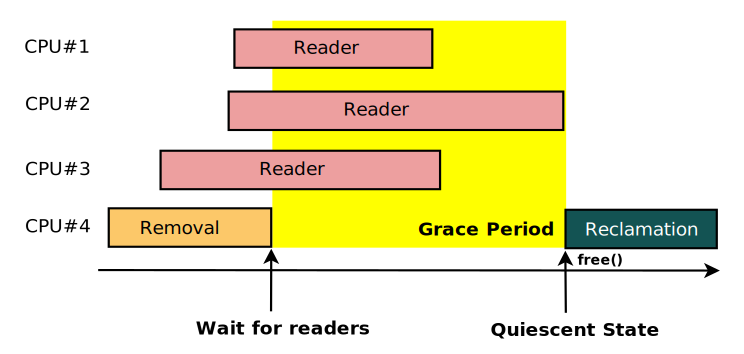
\includegraphics[width=1\textwidth]{fig/rcu/rcu_grace}
    \caption{RCU의 delayed free의 시점}
  \label{fig:rcu_grace}
\end{figure}

%$$$$$$$$$$$$$$$$$$$$$$$$$$$$$$$$$$$$$$$$$$$$$$$$$$$$$$$$$$$$$$$$$$$$$$$$$$$$$$$$
%Paragraph 2: RCU의 grace periad
%$$$$$$$$$$$$$$$$$$$$$$$$$$$$$$$$$$$$$$$$$$$$$$$$$$$$$$$$$$$$$$$$$$$$$$$$$$$$$$$$
그림~\ref{fig:rcu_grace}는 RCU의 \code{delayed free}의 시점을 보여준다.
그림에서 \code{Removal} 명령이 도착하면  RCU는 \code{Removal} 명령을 수행하고 기다린다.  
그 이유는 그 동안 해당 데이터는 리더들이 사용하고 있을 가능성이 있기 때문이다.
그 시점 부터 \textit{grace period} 라고 부르는 리더들이 종료되기를 기다리고, \textit{quiescent
state}라고 부르는 예전 데이터를 읽고 있는 리더들이 없는 상태가 되면 그 때 \code{free()}를 수행한다. 
아직 RCU는 리눅스 스케줄러에 의존하여 \textit{quiescent state}를 판단하나, 
이것은 \textit{grace period}가 길어 질 수 있어 문제가 있다. 
최근에는 이러한 문제를 해결하기 위해 \textit{quiescent state}를 마지막 리더가 끝나는 순간 바로 판단할 
수 있는 방법~\cite{Arbel2015PRR}이 연구되고 있다.

\subsubsection{RLU}

%$$$$$$$$$$$$$$$$$$$$$$$$$$$$$$$$$$$$$$$$$$$$$$$$$$$$$$$$$$$$$$$$$$$$$$$$$$$$$$$$
%Paragraph : RLU가 해결하고자 하는 문제
%$$$$$$$$$$$$$$$$$$$$$$$$$$$$$$$$$$$$$$$$$$$$$$$$$$$$$$$$$$$$$$$$$$$$$$$$$$$$$$$$
RLU는 \textit{Alexander Matveev외}가 RCU의 문제점을 해결한 연구이다. 
RCU는 Read-mostly 자료구조에 적합한 방법이나, RCU를 사용하기에는 프로그래머의 상당한 노력이 
필요하고, 라이터들이 증가할 수 록 높은 오버헤드를 가지는 단점이 있다.
또한 RCU의 \code{delayed free}는 모든 리더가 종료했을 때 바로 \code{quiescent state}를 찾는 것이 아니기
때문에 시간에 민감한 응용프로그램에 문제를 가진다. 
이러한 문제를 해결하기 위해 만든 것이 RLU~\cite{Matveev2015RLU}이다. 
RLU는 업데이트 문제를 해결한 로그 기반 알고리즘이나, 
이것은 Read-mostly 자료구조에서 라이터의 원자적 명령어에 의한 오버헤드가 심한 문제를 
싱글 원자적 연산을 사용한 Global Clock 변수와 오브젝트 레벨 안에 퍼코어 단위로 로깅을 사용한 방법을 사용한다.
따라서 업데이트가 많아지면 여전히 확장성 문제가 발생한다. 

\subsubsection{논블락킹(Non-blocking) 동기화}

%$$$$$$$$$$$$$$$$$$$$$$$$$$$$$$$$$$$$$$$$$$$$$$$$$$$$$$$$$$$$$$$$$$$$$$$$$$$$$$$$
%Paragraph : Non-locking synchronization의 장점
%$$$$$$$$$$$$$$$$$$$$$$$$$$$$$$$$$$$$$$$$$$$$$$$$$$$$$$$$$$$$$$$$$$$$$$$$$$$$$$$$
논블락킹 동기화 방법의 장점은 여러 스레드들이 락 기반으로 자원을 관리함에 따라 
발생하는 여러 문제를 해결할 수 있다.
가장 큰 장점은 스레드 또는 프로세스가 락 때문에 기다리는 시간을 제거할 수 있다.
이 것은 락을 얻기 위해 기다리는 시간을 최소화 할 뿐만 아니라 무한 루프 때문에 특정 스레드가 무한정 기다리는 
데드락(deadlock) 상황까지 제거 할 수 있다. 
다음으로 앞에서 설명하였듯이 코어 수가 증가 할 수록 락 자체를 얻기 위해 원자적 명령을 이용하는데 이것은 
캐시 일관성 트래픽을 발생한다. 
논블락킹 방법들은 이러한 락 오버헤드 자체를 제거할 수 있다. 
이와 같이 논블락킹 방법은 락 자체가 가지고 있는 문제점인 데드락, 라이브락(Livelock), 
우선순위 역전 현상(Priority Inversion)등을 한번에 제거 할 수 있다. 
또한 논블락킹 동기화 기법을 사용하는 \code{lock-free} 자료 구조들은 성능을 향상 시킬 수 있는데, 
그 이유는 멀티코어 환경에서 공유되는 데이터를 접근하기 위해 여러 스레드가 마치 바쁜대기 처럼 동작하므로 
직렬화 되는 부분이 매우 짧다.

\begin{figure}[h!]
    \centering
    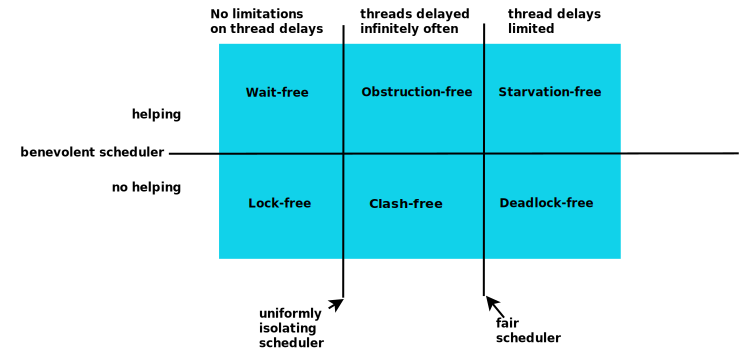
\includegraphics[width=1\textwidth]{fig/NBS/NBS}
    \caption{Non-blocking 동기화 기법의 분류}
  \label{fig:NBS}
\end{figure}


%$$$$$$$$$$$$$$$$$$$$$$$$$$$$$$$$$$$$$$$$$$$$$$$$$$$$$$$$$$$$$$$$$$$$$$$$$$$$$$$$
%Paragraph : Non-locking synchronization 알고리즘 종류 1 
%$$$$$$$$$$$$$$$$$$$$$$$$$$$$$$$$$$$$$$$$$$$$$$$$$$$$$$$$$$$$$$$$$$$$$$$$$$$$$$$$
이러한 논블락킹 동기화 기법은 그림~\ref{fig:NBS}와 같이 분류된다.
크게 보면 \textit{Wait-free}방법과 \textit{Lock-free}으로 구분되고, 이것은 1990대 초에 구분되었다.  
\textit{Wait-free} 방법은 가장 구현하기 힘든 알고리즘이며, 모든 스레드가 딜레이 없이 바로 종료할 수 
있는 알고리즘이다. 
다음으로 \textit{Lock-free} 방법은 적어도 하나의 스레드는 딜레이 없이 바로 끝나는 방법이다. 
즉 그 이외의 스레드들은 전역 변수를 동시에 접근해서 발생하는 충돌 때문에 다시 순회할 가능성이 있는 
알고리즘이다.

\begin{figure}[h!]
\begin{center}
\inputminted[linenos,fontsize=\footnotesize,
tabsize=4]{c}{src/lockfree_stack.c}
\end{center}
\caption{간단한 Non-blocking 스택 알고리즘.}
\label{fig:nonblockingstack}
\end{figure}


%$$$$$$$$$$$$$$$$$$$$$$$$$$$$$$$$$$$$$$$$$$$$$$$$$$$$$$$$$$$$$$$$$$$$$$$$$$$$$$$$
%Paragraph : 심플 스택 알고리즘 설명
%$$$$$$$$$$$$$$$$$$$$$$$$$$$$$$$$$$$$$$$$$$$$$$$$$$$$$$$$$$$$$$$$$$$$$$$$$$$$$$$$
이러한 장점을 가진 논블락킹 알고리즘의 스택의 예는 그림 \ref{fig:nonblockingstack}과 같이
구현되어 있다.
자료구조(\code{struct element})의 내용은 \code{value}와 다음 노드를 가리키는 포인터(Line 4)가 존재한다.
\code{push} 함수 같은 경우를 보면, 먼저 새로운 노드의 스택의 \code{top}에 해당하는 노드를 저장(Line 12)하고, 
CAS 연산을 통해 원자적으로 수정되었는지 체크를 함과 동시에 스택의 top에 해당하는 노드를 새로운 노드로 수정한다.
만약 CAS 연산이 실패하였다면(Line 13) 이 경우는 다른 스레드가 수정하였다는 것을 의미한다.
따라서 다시 처음 작업으로 이동(Line 11) 후 앞에서 수행한 일을 반복하여 수행한다.
\code{pop} 함수는 먼저 스택의 \code{top}에 해당하는 포인터를 지역 변수에 저장 후(Line 20), CAS 연산을 통해 
원자적으로 top 다음 포인터를 가르키게 한 후(Line 21) top에 해당하는 노드를 반환한다(Line 23). 
만약 CAS 연산이 실패하면 \code{push} 처럼 처음 부터 같은 일을 반복 수행한다(Line 19).

%$$$$$$$$$$$$$$$$$$$$$$$$$$$$$$$$$$$$$$$$$$$$$$$$$$$$$$$$$$$$$$$$$$$$$$$$$$$$$$$$
%Paragraph : ABA 문제 설명
%$$$$$$$$$$$$$$$$$$$$$$$$$$$$$$$$$$$$$$$$$$$$$$$$$$$$$$$$$$$$$$$$$$$$$$$$$$$$$$$$
논블락킹 동기화 기법의 가장 큰 현실적인 문제점은 바로 중간에 노드의 메모리 주소가 
바뀔 수 있다는 것이다. 
예를 들어 스택에 \code{top->A->B->C}세가지 노드가 순차적으로 들어 있을 경우, 
CPU\#1이 A를 꺼내고자 top의 포인터를 B를 가리키기 위해서 \code{CAS(top, A, B)} 연산을 
수행하는 순간 바로 선점 되어,  
CPU\#2가 A와 B를 꺼내고 그 A, B를 \code{free}한 후 다시 새로운 값과 함께 전에 사용한 A 주소를 재 사용하고, 
스택에 넣으면, 결국 CPU\#1의 \code{CAS(top, A, B)} 명령어는 성공하게 된다.
따라서 원하는 스택의 결과는 \code{top->C}을 얻어야 하는데, 그렇지 않고 \code{top->B->C} 순서로 스택에 쌓이게
된다.
이러한 상황을 ABA 문제라고 한다. 
이러한 문제의 간단한 해결책은 \code{free()}를 바로 호출하지 않고, 레퍼런스 카운트를 보고 해제하거나, 
안전한 시간(모든 프로세서가 작업이 끝날 때)까지 기다린 후 호출하는 방법이 있다. 

\subsection{확장성 있는 자료구조}

\subsubsection{Harris Linked List}

%$$$$$$$$$$$$$$$$$$$$$$$$$$$$$$$$$$$$$$$$$$$$$$$$$$$$$$$$$$$$$$$$$$$$$$$$$$$$$$$$
%Paragraph 2: harris 알고리즘 설명
%$$$$$$$$$$$$$$$$$$$$$$$$$$$$$$$$$$$$$$$$$$$$$$$$$$$$$$$$$$$$$$$$$$$$$$$$$$$$$$$$
논블락킹 알고리즘 중 대표적인 알고리즘 중 하나는 2001년도에 발표된 Harris Linked
List~\cite{Harris2001Lockfree}이다.
Harris 알고리즘은 CAS를 이용한 대표적인 알고리즘 중 하나이며, 순서대로 정렬된 노드들을 순회하면서 해당 
노드의 위치의 오른쪽 노드를 찾은 후 CAS로 새로운 노드를 삽입하는 방법이다. 

\begin{figure}[h!]
    \centering
    \includegraphics[width=1\textwidth]{fig/harris/harris}
    \caption{Harris 삭제}
  \label{fig:harris}
\end{figure}


%$$$$$$$$$$$$$$$$$$$$$$$$$$$$$$$$$$$$$$$$$$$$$$$$$$$$$$$$$$$$$$$$$$$$$$$$$$$$$$$$
%Paragraph 2: 그림 설명
%$$$$$$$$$$$$$$$$$$$$$$$$$$$$$$$$$$$$$$$$$$$$$$$$$$$$$$$$$$$$$$$$$$$$$$$$$$$$$$$$
이러한 Hariis 알고리즘의 한 예인 삭제 연산에 대해서 설명하면 그림~\ref{fig:harris}과 같다. 
시간 순서 대로 위에서 아래로 진행된다.
동시에 \code{CORE\#1}이 노드 B를 삭제하고 \code{CORE\#2}가 노드 C를 삭제한다면,
Harris 링크드 리스트에서는 삭제를 바로 수행하지 않고, 먼저 각 노드에 마킹을 한다. 
Harris 링크드 리스트 알고리즘은 이것을 \code{logical remove}라고 한다.
다음으로 \code{CORE\#1}과 \code{CORE\#2}가 동시에 CAS 연산을 사용하여 삭제를 하면, \code{CORE\#2}의
오래된 값이 \code{CORE\#1}에 의해 변경되었기 때문에 이 순간 CAS 실패가 발생하다. 
CAS 실패에 의해 논리적으로 삭제가 되었지만 아직 물리적으로 노드가 남아 있는 상태가 되었기 때문에, 
Harris 리스트는 CAS가 실패하면
처음 부터 다시 순회하고, 마킹된 노드를 다시 CAS 연산을 사용해 제거한다.
Harris 리스트의 오버헤드는 CAS 연산, \code{logical remove}에 따른 전역 변수의 수정, 그리고 
수정된 노드들을 각 코어들이 CAS 실패 할 때 마다 다시 순회를 함에 따라 
캐시 일관성 트래픽이 많이 발생하여 성능에 문제가 있다.

%\subsubsection{Time-stamp stack}


